\documentclass[11pt,class=report,crop=false]{standalone}
\usepackage[screen]{../python}


\begin{document}

%====================================================================
\chapitre{Big data I}
%====================================================================

\index{big data@\emph{big data}}


\objectifs{\emph{Big data}, intelligence artificielle, \emph{deep learning}, réseau de neurones,  \emph{machine learning}\ldots{} plein de mots compliqués ! Le but commun est de faire exécuter à un ordinateur des tâches de plus en plus complexes : \emph{choisir} (par exemple trouver un bon élément parmi des milliards selon plusieurs critères), \emph{décider} (séparer des photos de chats de photos de voitures), \emph{prévoir} (un malade a de la fièvre et le nez qui coule, quelle maladie est la plus probable ?).
Dans cette première partie, on va utiliser des outils classiques de statistique et de probabilité pour résoudre des problèmes amusants.}

\bigskip


%%%%%%%%%%%%%%%%%%%%%%%%%%%%%%%%%%%%%%%%%%%%%%%%%%%%%%%%%%%%%%%%
%%%%%%%%%%%%%%%%%%%%%%%%%%%%%%%%%%%%%%%%%%%%%%%%%%%%%%%%%%%%%%%%

\begin{cours}[Des données par milliers]

Lorsque l'on parle de \emph{big data} on parle de fichiers avec des milliards de données.
On va plus modestement traiter de fichiers contenant les données (fictives) de $100\,000$ personnes.

Récupères le fichier \ci{personnes_100000.csv}. Tu disposes aussi des fichiers \ci{personnes_100.csv}, \ci{personnes_1000.csv}, \ci{personnes_10000.csv} qui contiennent moins d'entrées et sont idéaux pour tester les programmes.

\smallskip

Ces fichiers sont disponibles ici :
\mycenterline{\href{https://github.com/exo7math/python2-exo7}{github.com/exo7math/python2-exo7}}

\bigskip

Voici un exemple de ligne de ce fichier au format \emph{csv} (\emph{comma separated values}):
\mycenterline{\ci{femme,Lessard,Capucine,7/31/1978,LA ROCHELLE,56.7,155,O+}}
ou 
\mycenterline{\ci{homme,Cadieux,Antoine,11/20/1938,METZ,78.8,166,A-}}

\medskip

Chaque ligne désigne une personne et ses caractéristiques :
\begin{itemize}
	\item sexe (homme/femme)
	\item nom
	\item prénom
	\item date de naissance (format jj/mm/aaaa)
	\item ville
	\item poids (en kilogrammes)
	\item taille (en centimètres)
	\item groupe sanguin
\end{itemize}

\end{cours}



%%%%%%%%%%%%%%%%%%%%%%%%%%%%%%%%%%%%%%%%%%%%%%%%%%%%%%%%%%%%%%%%
% Activité 1 - Sondage
%%%%%%%%%%%%%%%%%%%%%%%%%%%%%%%%%%%%%%%%%%%%%%%%%%%%%%%%%%%%%%%%

\begin{activite}[Sondage]
	
\objectifs{Objectifs : utiliser un échantillon pour déterminer les caractéristiques d'une population.}
		
\begin{enumerate}
	\item Programme une fonction \ci{age_moyen(debut,fin,fichier)} qui évalue l'âge moyen d'une liste de personnes (contenue dans le fichier donné)
	à partir d'un échantillon.
	Par exemple :
	\ci{age_moyen(10,20,"personnes_100.csv")}
	renvoie la moyenne des âges des personnes de rang $10$ (compris) à $20$ (exclu) parmi une liste de $100$ personnes.
	
	\emph{Indication.} L'âge d'une personne est l'âge qu'elle aura à la fin de l'année en cours.
	
	Compare l'âge moyen calculé à partir de l'échantillon avec l'âge moyen de toute la liste. Quelle taille de l'échantillon permet d'avoir une estimation à $1$ an près ?
	
	\item Programme une fonction \ci{probabilite_initiale(lettre,debut,fin,fichier)}
	qui estime la probabilité que le nom d'une personne commence par la lettre donnée à partir d'un échantillon de la liste.
	Pour cela on approche la probabilité par la formule :
	$$\text{probabilité} \quad \simeq \quad \frac{\text{nombre d'occurences}}{\text{nombre total d'éléments}}$$
	
	\item Programme une fonction \ci{probabilite_groupe_sanguin(debut,fin,fichier)} qui renvoie les probabilités de chaque groupe sanguin. La fonction renvoie un dictionnaire dont le couple \og{}clé/valeur\fg{} est \og{}groupe sanguin/probabilité\fg{}.
	Les groupes possibles sont A+, A-, B+, B-, O+, O-, AB+ et AB-.
	Par exemple (obtenu sur un échantillon de $10$ personnes seulement) :
	
	\mycenterline{\ci{\{ 'A+': 0.1, 'A-': 0.1, 'B+': 0.1, 'B-': 0.1,}}
	\mycenterline{\ci{   'O+': 0.3, 'O-': 0.3, 'AB+': 0.0, 'AB-': 0.0 \}}}
	
	Quels sont les groupes les plus fréquents ?
	
\end{enumerate}
		
\end{activite}


%%%%%%%%%%%%%%%%%%%%%%%%%%%%%%%%%%%%%%%%%%%%%%%%%%%%%%%%%%%%%%%%
%%%%%%%%%%%%%%%%%%%%%%%%%%%%%%%%%%%%%%%%%%%%%%%%%%%%%%%%%%%%%%%%

\begin{cours}[Ordre alphabétique]
On rappelle que \Python{} connaît l'ordre alphabétique et qu'on peut comparer deux chaînes de caractères :
\begin{itemize}
	\item \og{}\ci{"A" < "B"}\fg{} est \og{}Vrai\fg{} (\Python{} renvoie \ci{True}),
	\item \og{}\ci{"BAC" < "ABC"}\fg{} est \og{}Faux\fg{},
	\item \og{}\ci{"A" == "a"}\fg{} est \og{}Faux\fg{}.
\end{itemize}

Tu peux consulter la fiche \og{}Le mot le plus long\fg{} et aussi la fiche \og{}Tri - Complexité\fg{} pour plus d'informations 
et une activité similaire à l'activité suivante.
\end{cours}


%%%%%%%%%%%%%%%%%%%%%%%%%%%%%%%%%%%%%%%%%%%%%%%%%%%%%%%%%%%%%%%%
% Activité 2 - Chercher dans une liste de noms
%%%%%%%%%%%%%%%%%%%%%%%%%%%%%%%%%%%%%%%%%%%%%%%%%%%%%%%%%%%%%%%%

\begin{activite}[Chercher dans une liste de noms]
	
	\objectifs{Objectifs : chercher dans une liste élément par élément ou bien par dichotomie.}
	
	
	\begin{enumerate}
		\item \textbf{Liste triée.}
		Programme une fonction \ci{fichier_vers_liste_noms(fichier)} qui renvoie la liste \emph{ordonnée} des noms issus du fichier.
		
		\emph{Indication.} \ci{liste.sort()} trie la liste.
		
		\item \textbf{Début d'une chaîne.}
		Programme une fonction \ci{est_debut(debut,chaine)} qui teste si une chaîne débute par les caractères donnés.
		Par exemple :
		\begin{itemize}
			\item \ci{est_debut("ABC","ABCDEF")} renvoie \og{}Vrai\fg{},
			\item \ci{est_debut("XYZ","ABCDEF")} renvoie \og{}Faux\fg{},
			\item \ci{est_debut("ABCD","AB")} renvoie \og{}Faux\fg{}.						
		\end{itemize}
	
		\item \textbf{Recherche séquentielle.}
		Programme une fonction \ci{chercher_1(liste,debut)}
		qui renvoie un nom de la liste commençant par \ci{debut} (ou \ci{None} si un tel nom n'existe pas). 
		
		\emph{Méthode.} Parcours un par un les noms de la liste (issue de la première question) et teste s'il commence par \ci{debut}.
		
		Par exemple \ci{chercher_1(liste,"Bri")} peut renvoyer \ci{'Brian'}.
		
		\item \textbf{Recherche dichotomique.}
		Programme une fonction \ci{chercher_2(liste,debut)} qui fait le même travail mais avec un algorithme plus efficace : la dichotomie.
		
		\begin{algorithme}
			\sauteligne 
			
			\begin{itemize}
				\item 
				\begin{itemize}
					\item Entrée : un début de mot à trouver et une liste ordonnée de noms.
					
					\item Sortie : un mot trouvé dans la liste commençant par le début souhaité ou \ci{None} en cas d'échec. 
					
				\end{itemize}
				
				\item $a \leftarrow 0$ (le rang d'une liste commence à $0$).
				
				\item $b \leftarrow n -1$ où $n$ est la longueur de la liste.
				
				\item Tant que $b \ge a$, faire :
				\begin{itemize}
					\item $k \leftarrow (a+b)//2$
					
					\item Si \ci{debut} est le début du mot \ci{liste[k]} alors renvoyer \ci{liste[k]}.
					\item Si \ci{debut} vient après \ci{liste[k]} dans l'ordre alphabétique alors faire $a\leftarrow k+1$,
					\item sinon faire $b \leftarrow k-1$.
				\end{itemize}
				
				\item Renvoyer \ci{None} (c'est le cas uniquement si aucun nom n'a été trouvé dans la boucle précédente).
				
			\end{itemize}
		\end{algorithme}  
	
		Par exemple \ci{chercher_2(liste,"Bri")} peut renvoyer \ci{'Brisebois'}.
		Le nom trouvé par cet algorithme n'est pas nécessairement le premier qui viendrait dans l'ordre alphabétique.
		
		\item \textbf{Complexité.}
		\begin{enumerate}
			\item Modifie tes deux fonctions de recherche pour qu'elles renvoient en plus du nom, le nombre d'itérations nécessaires (par exemple le nombre de fois où tu effectues un appel à la fonction \ci{est_debut()}).  
			
			\item Vérifie expérimentalement que si $n$ est la longueur de la liste ordonnée, alors :
			\begin{itemize}
				\item pour la recherche séquentielle, il peut y avoir jusqu'à $n$ itérations,
				\item pour la recherche par dichotomie, il peut y avoir jusqu'à $E(\log_2(n)+1)$ itérations (où $E(x)$ désigne la partie entière, comme la commande \ci{floor(x)}).
			\end{itemize}
		\end{enumerate}
		

		
		
	\end{enumerate}
	
\end{activite}




%%%%%%%%%%%%%%%%%%%%%%%%%%%%%%%%%%%%%%%%%%%%%%%%%%%%%%%%%%%%%%%%
% Activité 3 - La formule des tanks
%%%%%%%%%%%%%%%%%%%%%%%%%%%%%%%%%%%%%%%%%%%%%%%%%%%%%%%%%%%%%%%%

\begin{activite}[La formule des tanks]
	
	\objectifs{Objectifs : déterminer la taille $N$ d'une série $1,\ldots,N$ en ne connaissant que quelques numéros tirés au hasard.}
	
	En plein milieu de la seconde guerre mondiale les Allemands produisent un nouveau tank plus performant. Les Alliés s'inquiètent car ils ne savent pas combien de ces nouveaux tanks sont produits. Les services de renseignements estiment la production à $1500$ tanks par mois. Que disent les mathématiques ?	
	Les Alliés ont intercepté $4$ tanks produits le même mois et qui portent les numéros :
	$$143 \qquad 77 \qquad 198 \qquad 32$$
	Combien de tanks ont été produit ce mois ?
	
	\emph{Modélisation.} 
	Sachant que les tanks sont numérotés de $1$ à $N$ chaque mois, à quelle valeur peut être estimée la production mensuelle $N$, connaissant un échantillon de $k$ numéros $[n_1,n_2,\ldots,n_k]$ ?
	
	
	
	\begin{enumerate}
		\item \textbf{La formule des tanks.}
		On note $m$ le maximum des éléments de l'échantillon. 
		On note $k$ la taille de l'échantillon.
		Alors la formule des tanks estime :
		$$N \simeq m + \frac{m}{k}-1$$
		
		Programme cette formule en une fonction \ci{formule_tanks(echantillon)} qui renvoie cette estimation de $N$.		
		Quelle est ton estimation pour le nombre de tanks ?
		
			
		\item \textbf{Le double de la moyenne.}
		On peut essayer d'autres estimations. Par exemple on peut estimer $N$ comme le double de la moyenne de l'échantillon.
		Programme une fonction \ci{double_moyenne(echantillon)} qui renvoie cette nouvelle estimation.		
		Compare avec la formule des tanks.
		
		\bigskip
		
		Pour tester l'efficacité de la formule des tanks on va faire le cheminement inverse : on fixe un entier $N$, on choisit au hasard un échantillon de $k$ éléments et on regarde si nos formules permettent de bien approcher $N$.
		
		\item \textbf{Tirage sans remise.}
		Programme une fonction \ci{tirage_sans_remise(N,k)} qui renvoie une liste de $k$ entiers différents compris entre $1$ et $N$ (inclus).
		
		\item \textbf{Erreurs.} Programme une fonction \ci{erreurs(N,k)}
		(ou mieux \ci{erreurs(N,k,nb_tirages=1000)}) qui calcule l'erreur moyenne commise par nos formules. 
		Pour cela :
		\begin{itemize}
			\item Effectue un tirage sans remise de $k$ entiers plus petits que $N$.
			\item Calcule la valeur $N_1$ obtenue à partir de cet échantillon par la formule des tanks.
			\item Calcule l'erreur commise $e = | N - N_1 |$. 
		\end{itemize}
		En faisant ceci pour un grand nombre de tirages, calcule l'erreur moyenne commise.
		Fais le même travail avec l'autre formule et renvoie les deux erreurs moyennes.
		
		Pour $20$ entiers plus petits que $1000$ ($k=20$ et $N=1000$) quelle est la meilleure formule et à quelle erreur peut-on s'attendre ?
		
	\end{enumerate}
	
	\`A la fin de la guerre les registres Allemands ont été récupérés et indiquaient une production de $245$ chars mensuels !
	Cette formule est aussi utilisée pour estimer la production d'un produit (par exemple d'un téléphone) à partir des numéros de série.
\end{activite}



%%%%%%%%%%%%%%%%%%%%%%%%%%%%%%%%%%%%%%%%%%%%%%%%%%%%%%%%%%%%%%%%
%%%%%%%%%%%%%%%%%%%%%%%%%%%%%%%%%%%%%%%%%%%%%%%%%%%%%%%%%%%%%%%%

\begin{cours}[Le problème du secrétaire]
	
La directrice d'une entreprise doit choisir son nouveau secrétaire : elle reçoit $k=100$ secrétaires un par un et attribue à chacun une note (par exemple un entier entre $0$ et $N=100$). Elle veut choisir le meilleur secrétaire mais il y a une contrainte : elle décide immédiatement après chaque entretien si elle embauche ou pas ce secrétaire. Elle n'a pas la possibilité de revenir en arrière.

Voici la stratégie qu'elle adopte : elle commence par recevoir un certain nombre de candidats (par exemple $25$), elle mémorise juste la meilleure note obtenue jusqu'ici sans retenir aucun de ces candidats. Ensuite elle reçoit les candidats suivants et elle sélectionne le premier qui a une note supérieure ou égale à la meilleure note de l'échantillon. Avec cette stratégie elle n'est pas sûre de trouver le meilleur secrétaire, et elle peut même ne sélectionner aucun secrétaire.

\bigskip

\emph{Exemple.}
Voici une liste de scores des candidats (ici avec seulement $10$ candidats) :\\
\mycenterline{\ci{liste = [2,5,3,4,1,6,4,5,8,3]}}
Prenons le pourcentage $p=25$.
La taille de la liste est $k=10$ donc l'échantillon de $25\%$
est formé des $2$ premiers éléments $[2,5]$. Le score maximum de cet échantillon est $M=5$. La directrice ne retient pas de candidat dans l'échantillon, par contre elle va  choisir le premier candidat suivant dont la note sera supérieure ou égal à $M$ et arrête le processus. Ici c'est donc le candidat avec un score de $6$ qui est choisi. Note qu'elle n'a pas sélectionné le meilleur candidat avec un score de $8$ mais qui était en fin de liste.
Le but est de choisir la bonne taille pour l'échantillon : avec un échantillon trop petit elle va choisir un secrétaire moyen, avec un échantillon trop grand elle ne va pas trouver de secrétaire du tout.

\bigskip

\emph{Notations.}
\begin{itemize}
	\item Le nombre de candidats secrétaires est $k$. Par défaut $k=100$.
	\item Les notes vont de $0$ à $N$. Par défaut $N=100$.
	\item La taille de l'échantillon s'exprime comme un pourcentage $p$ du nombre total de candidats $k$ total. Par exemple $p=25$ signifie que l'on teste d'abord $25\%$ de candidats.
\end{itemize}	
\end{cours}




%%%%%%%%%%%%%%%%%%%%%%%%%%%%%%%%%%%%%%%%%%%%%%%%%%%%%%%%%%%%%%%%
% Activité 4 - Le problème du secrétaire 
%%%%%%%%%%%%%%%%%%%%%%%%%%%%%%%%%%%%%%%%%%%%%%%%%%%%%%%%%%%%%%%%

\begin{activite}[Le problème du secrétaire]
	
	\objectifs{Objectifs : programmer la sélection d'un bon secrétaire et optimiser la taille de l'échantillon.}
	
\begin{enumerate}
	\item Programme une fonction \ci{genere_liste(k,N)} qui génère une liste de $k$ entiers 
	tirés au hasard entre $0$ et $N$ (deux nombres peuvent être identiques).		
	Cela correspond aux notes des $k$ secrétaires.
	
	\item Programme une fonction \ci{choix_secretaire(liste,p)} qui à partir d'une liste de notes et un pourcentage renvoie le score du secrétaire choisi (ou \ci{None} si aucun ne convient).
	La méthode adoptée est celle décrite dans le cours au-dessus:
	\begin{itemize}
		\item à partir de l'échantillon formé par les premiers candidats (la taille de l'échantillon est donnée sous la forme d'un pourcentage \ci{p}) on retient le meilleur score $M$ de cet échantillon, mais aucun n'est sélectionné,
		\item en recevant un par un les candidats suivants, on prend le premier ayant un score supérieur ou égal à $M$,
		\item si aucun ne convient on renvoie \ci{None}.
	\end{itemize}
	

	\item On souhaite savoir si notre stratégie est efficace ou pas : combien de fois sélectionne-t-on le meilleur secrétaire possible ?
	Pour cela tu vas tester la méthode sur un grand nombre de tirages.
	
	
    Programme une fonction \ci{meilleurs_secretaires(k,N,p,nb_tirages)}
	qui renvoie le nombre de fois où l'algorithme de la directrice sélectionne le meilleur candidat.
	\begin{itemize}
		\item $k$ est la longueur des listes,
		\item chaque note est un entier entre $0$ et $N$ (inclus),
		\item $p$ est le pourcentage qui détermine la taille de l'échantillon,
		\item \ci{nb_tirages} est le (grand) nombre de listes aléatoires à tester.
	\end{itemize}

	Par exemple avec $k=100$, $N=100$ et le pourcentage $p=25$ en effectuant de nombreux tirages (au moins $1000$) le candidat sélectionné est dans environ $47\%$ des cas le meilleur des candidats de toute la liste.
	
	\item Le pourcentage de $25\%$ pour l'échantillon n'est pas celui qui conduit aux meilleurs résultats. \'Ecris un programme ou bien tâtonne pour trouver la meilleure valeur de $p$ possible.
	
	\emph{Indice.} La réponse s'appelle la loi en $1/e$ !
\end{enumerate}
	
\end{activite}



%%%%%%%%%%%%%%%%%%%%%%%%%%%%%%%%%%%%%%%%%%%%%%%%%%%%%%%%%%%%%%%%
%%%%%%%%%%%%%%%%%%%%%%%%%%%%%%%%%%%%%%%%%%%%%%%%%%%%%%%%%%%%%%%%

\begin{cours}[Régression linéaire]

On se donne des points $(x_i,y_i)_{1\le i \le n}$. 
On cherche si on peut modéliser la situation par une relation linéaire entre l'abscisse et l'ordonnée du type :
$$y = ax+b$$



C'est-à-dire que l'on cherche la droite qui \og{}approche\fg{} au mieux tous les points.
Cette opération s'appelle la \defi{régression linéaire} et la droite est la \defi{droite des moindres carrés}.

Sur la figure ci-dessous à gauche une série de points $(x_i,y_i)$, à droite la droite des moindres carrés d'équation $y=ax+b$.
\begin{center}
	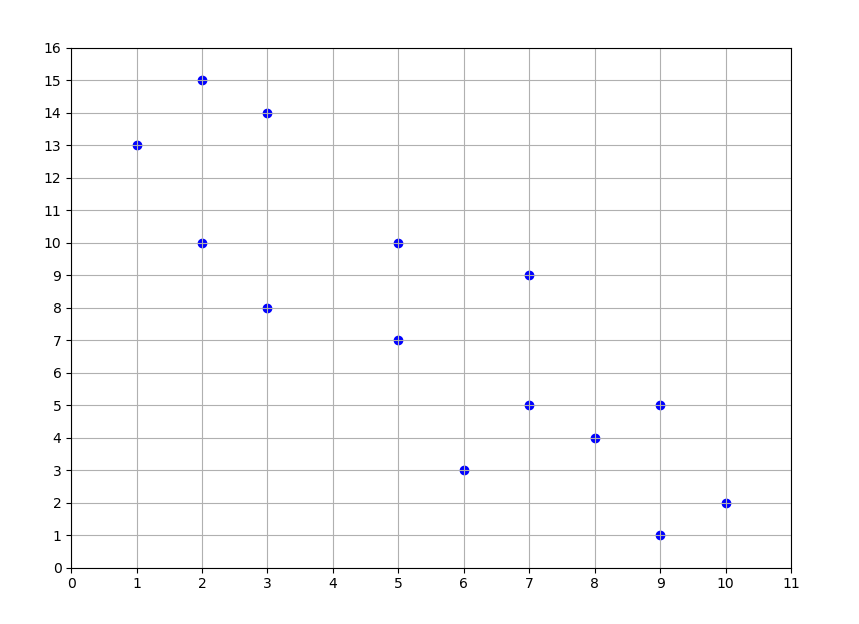
\includegraphics[scale=\myscale,scale=0.25]{cours-regression-1}	\quad
	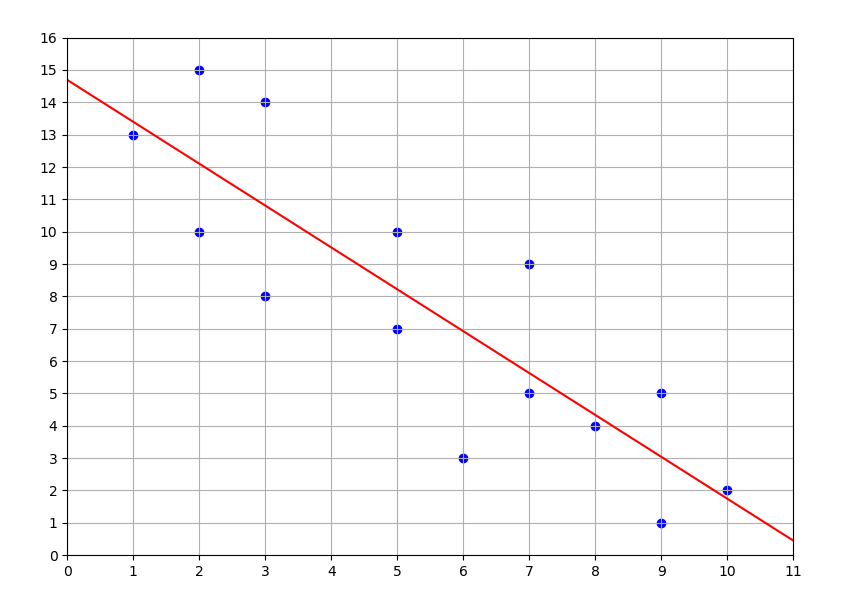
\includegraphics[scale=\myscale,scale=0.25]{cours-regression-2}
\end{center}


Voici comment calculer les coefficients $a$ et $b$ de la droite $y=ax+b$.
\begin{itemize}
	\item On note $m_x$ la moyenne des $(x_i)_{1\le i \le n}$. 
	
	\item On note $m_y$ la moyenne des $(y_i)_{1\le i \le n}$. 	
	
	\item On note $\operatorname{Var}(x)$ la \defi{variance} des $(x_i)_{1\le i \le n}$ :
	$$\operatorname{Var}(x) = \frac{1}{n} \sum_{i=1}^{n}(x_i-m_x)^2$$
	c'est-à-dire:
	$$\operatorname{Var}(x) = \frac1n\left((x_1-m_x)^2 + (x_2-m_x)^2 + \cdots + (x_n-m_x)^2\right)$$
	
	La variance mesure l'écart des valeurs avec la moyenne.
	La variance est aussi le carré de l'écart-type.
	
	\item On note $\operatorname{Cov}(x,y)$ la \defi{covariance} des $(x_i)_{1\le i \le n}$ avec $(y_i)_{1\le i \le n}$ :
	$$\operatorname{Cov}(x,y) = \frac{1}{n} \sum_{i=1}^{n}(x_i-m_x)(y_i-m_y)$$
	c'est-à-dire:
	$$\operatorname{Cov}(x,y) = \frac1n\left((x_1-m_x)(y_1-m_y) + (x_2-m_x)(y_2-m_y) + \cdots + (x_n-m_x)(y_n-m_y)\right)$$
	
	La covariance mesure la corrélation (c'est-à-dire la dépendance) entre les valeurs $x_i$ et $y_i$.
	
	\item Alors les coefficients de la droite $y=ax+b$ sont :
	$$a =  \frac{\operatorname{Cov}(x,y)}{\operatorname{Var}(x)}
	\qquad \text{ et } \qquad
	b = m_y - a m_x$$
	
\end{itemize}

	
\end{cours}


%%%%%%%%%%%%%%%%%%%%%%%%%%%%%%%%%%%%%%%%%%%%%%%%%%%%%%%%%%%%%%%%
% Activité 5 - Régression linéaire
%%%%%%%%%%%%%%%%%%%%%%%%%%%%%%%%%%%%%%%%%%%%%%%%%%%%%%%%%%%%%%%%

\begin{activite}[Régression linéaire]
	
\objectifs{Objectifs : tracer la droite des moindres carrés.}

\begin{enumerate}
	\item \textbf{Moyenne, variance, covariance.}
	
	Programme :
	\begin{itemize}
		\item une fonction \ci{moyenne(liste)} qui renvoie la moyenne des éléments $(x_i)$ de la liste,
		
		\item une fonction \ci{variance(liste)} qui renvoie la variance des éléments $(x_i)$ de la liste,
		
		\item une fonction \ci{covariance(listex,listey)} qui renvoie la covariance des éléments $(x_i)$ et $(y_i)$.
	\end{itemize}
	
	\emph{Exemples.}
	\begin{itemize}
		\item Vérifie que la moyenne de $(1,2,3,4,5)$ est $m_x = 3$ et la variance $\operatorname{Var}(x) = 2$.
		
		\item Vérifie que la covariance entre $(1,2,3,4,5)$ et $(4,5,4,7,6)$ vaut $\operatorname{Cov}(x,y) = 1.2$.
		
		\item Vérifie sur un exemple que $\operatorname{Cov}(x,x) = \operatorname{Var}(x)$.
	\end{itemize}	

	\item \textbf{Régression linéaire.}
	
	Programme une fonction \ci{regression_lineaire(points)} qui à partir d'une liste de points
	$(x_i,y_i)_{1\le i \le n}$ renvoie les coefficients $a,b$ de la droite d'équation $y = ax+b$.
	
	\emph{Exemple.}
	Pour le bac blanc on a demandé à chaque élève le temps qu'il a passé pour ses révisions (valeur $x_i$) et la note qu'il a obtenue (valeur $y_i$).
	
	Voici la liste $(x_i,y_i)$ des données, par exemple le premier élève à réviser $0.25$ heures et a obtenu $5$,
	le dernier à réviser $3$ heures et a obtenu $16$.
\begin{center}
\begin{minipage}{0.85\textwidth}	
\begin{lstlisting}		
eleves = [ (0.25,5), (0.5,4), (0.75,7), (1,6), (1,7),
          (1,10), (1.5,9), (1.75,14), (2,9), (2,11), (2.25,15),
          (2.5,10), (2.5,13), (2.75,18), (3,13), (3,16) ]
\end{lstlisting}
\end{minipage}
\end{center}
   Calcule les coefficients $a$ et $b$ associés à la régression linéaire.
	
	Voici ces points, en abscisse le temps de travail (en heures) et en ordonnée la note obtenue (sur $20$) :
	\begin{center}
		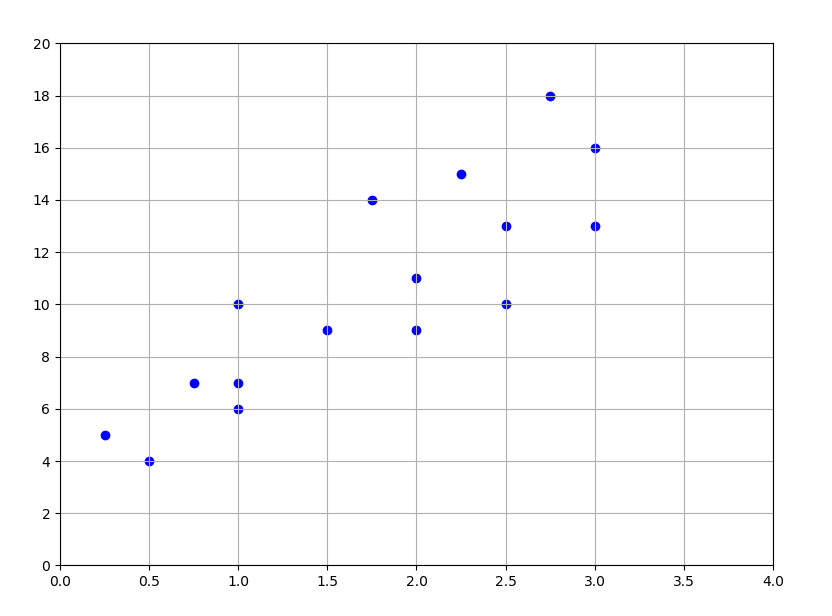
\includegraphics[scale=\myscale,scale=0.3]{ecran-regression-1}	
	\end{center}
	 
	J'ai révisé pendant $2$ heures, quelle note puis-je espérer ?
	\item \textbf{Affichage.}
	
	Programme une fonction \ci{afficher(points)} qui réalise l'affichage des points et de la droite des moindres carrés d'équation $y = ax+b$.
	\begin{center}
	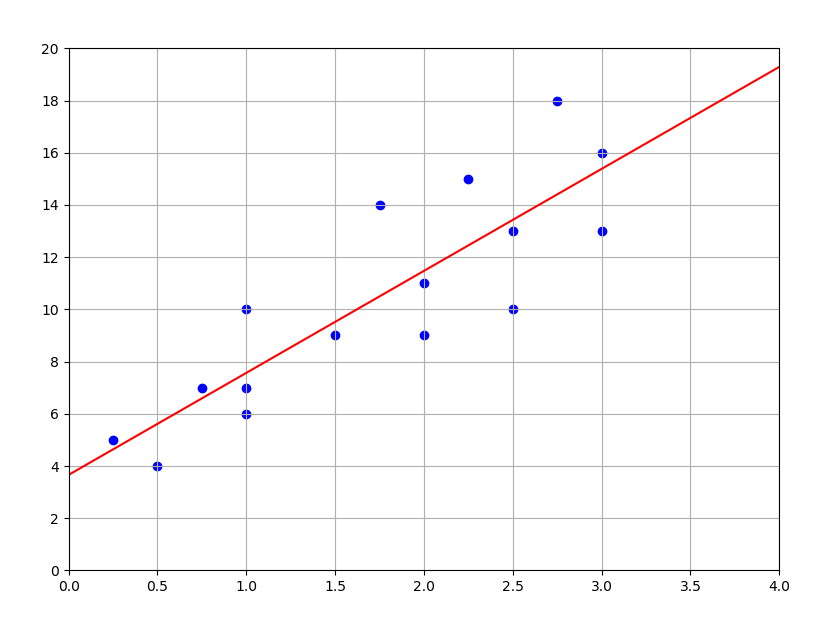
\includegraphics[scale=\myscale,scale=0.3]{ecran-regression-2}	
	\end{center}	

	
	\item \textbf{Travailler plus pour gagner plus.}
	
	\'Ecris un petit programme qui demande à l'utilisateur \og{}Quelle note aimerais-tu avoir ?\fg{}
	et à partir de la réponse donnée affiche une phrase du type \og{}Tu dois travailler au moins 2 heures et 30 minutes.\fg{}. 
	
	\emph{Indications.} 
	\begin{itemize}
		\item \ci{input()} attend de l'utilisateur une réponse qui est renvoyée sous la forme d'une chaîne de caractères. 
		\item \ci{float(chaine)} transforme une chaîne en un nombre flottant, par exemple 
		\ci{float("12.5")} renvoie \ci{12.5}.
	\end{itemize}
\end{enumerate}
	
\end{activite}




%%%%%%%%%%%%%%%%%%%%%%%%%%%%%%%%%%%%%%%%%%%%%%%%%%%%%%%%%%%%%%%%
%%%%%%%%%%%%%%%%%%%%%%%%%%%%%%%%%%%%%%%%%%%%%%%%%%%%%%%%%%%%%%%%

\begin{cours}[Distribution de Gauss]

\textbf{Distribution de Gauss.}
	
Certaines données se répartissent suivant une \defi{distribution de Gauss} (appelée aussi \defi{loi normale}).
Une distribution de Gauss est déterminée par deux paramètres :
\begin{itemize}
	\item l'espérance (ou la moyenne) $\mu$,
	\item la variance (ou l’écart-type au carré) $\sigma^2$,
\end{itemize}
et se calcule par la formule :
$$p(x) = \frac{1}{\sqrt{2\pi\sigma^2}} \exp\left( -\frac12 \frac{(x-\mu)^2}{\sigma^2} \right)$$

Le graphe de cette fonction est une courbe en cloche, centrée sur l'espérance $\mu$, et qui s'étale plus ou moins en fonction de la variance $\sigma^2$.

\myfigure{0.6}{
	\tikzinput{fig_bigdata_01}\qquad
	\tikzinput{fig_bigdata_02}
}

\myfigure{0.6}{
	\tikzinput{fig_bigdata_03}
}

La fonction $x \mapsto p(x)$ s'appelle une \defi{densité de probabilité}. $p(x)$ n'est pas une probabilité et on peut avoir $p(x)>1$ pour certains $x$. Par contre l'aire sous la courbe vaut toujours $1$.

\bigskip

\textbf{Détermination de la distribution à partir d'un échantillon.}

Si on nous donne un échantillon de données $x_1,\ldots,x_n$ alors on peut lui associer une distribution de Gauss en prenant :
\begin{itemize}
	\item $\mu$ la moyenne de $x_i$,
	\item $\sigma^2$ la variance des $x_i$.
\end{itemize}

\medskip

\emph{Exemple de la taille.}
Voici une liste de tailles de $5$ hommes : $[181,170,186,175,169]$.
\`A partir de cet échantillon on calcule la moyenne $\mu_h = 176$ (arrondie à 1 cm près)
et $\sigma^2_h = 42$. (Tu calculeras les vraies valeurs dans l'activité suivante.)
On peut calculer la distribution de Gauss de la taille des hommes (voir le graphique ci-dessous).

On peut faire la même chose à partir de l'échantillon suivant de tailles de femmes : $[162,174,160,171,162]$. On trouve $\mu_f = 166$ et $\sigma^2_f = 32$.   

On obtient donc deux densités de probabilité : $p_f(x)$ pour les hommes et $p_f(x)$ pour les femmes.

\myfigure{0.55}{
	\tikzinput{fig_bigdata_04}\quad
	\tikzinput{fig_bigdata_05}
}

\bigskip

\textbf{Classification.}

On veut savoir si quelqu'un de taille $x=169$ cm est plutôt un homme ou une femme ?
On a donc deux densités de probabilité : on calcule $p_h(x)$ (comme si c'était un homme) et $p_f(x)$ (comme si c'était une femme) et on compare ces deux valeurs.
Si $p_h(x)>p_f(x)$ alors c'est plus probablement un homme, sinon c'est plutôt une femme. 

Ici on calcule $p_h(x) \simeq 0.035$ et $p_f(x) \simeq 0.061$, donc avec nos données, quelqu'un de $169$ cm est plus probablement une femme.

On peut aussi le voir graphiquement ci-dessous : pour $x=169$ la courbe des femmes est au-dessus de la courbe des hommes. 

\myfigure{1}{
	\tikzinput{fig_bigdata_06}
}

\end{cours}



%%%%%%%%%%%%%%%%%%%%%%%%%%%%%%%%%%%%%%%%%%%%%%%%%%%%%%%%%%%%%%%%
% Activité 6 - Classification bayésienne naïve
%%%%%%%%%%%%%%%%%%%%%%%%%%%%%%%%%%%%%%%%%%%%%%%%%%%%%%%%%%%%%%%%

\begin{activite}[Classification bayésienne naïve]
	
\objectifs{Objectifs : classer une donnée dans une catégorie ou une autre, par exemple décider si une personne est un homme ou une femme connaissant sa taille et son poids.}

\begin{enumerate}
	\item \textbf{Moyenne et variance.}
	Détermine la moyenne $\mu_h$ et la variance $\sigma^2_h$ de la taille des hommes à partir de cet échantillon de taille (en cm) :	
	\mycenterline{\ci{taille_hommes = [172,165,187,181,167,184,168,174,180,186]}}
	
	Même chose avec $\mu_f$ et $\sigma^2_f$ pour les femmes :	
	\mycenterline{\ci{taille_femmes = [172,156,164,182,171,164,162,170,161,167]}}
	
	\item \textbf{Densité de probabilité.}
	Programme une fonction \ci{densite_gauss(x,mu,sigma2)} qui renvoie
	$$p(x) = \frac{1}{\sqrt{2\pi\sigma^2}} \exp\left( -\frac12 \frac{(x-\mu)^2}{\sigma^2} \right)$$
	où \ci{mu}\,$=\mu$ est une espérance (notre moyenne) et \ci{sigma2}\,$=\sigma^2$ est une variance.
	

	\item \textbf{Homme ou femme par la taille.}
	
	On donne la taille $x$ d'une personne, par exemple $x=170$, on souhaite savoir si cette personne est plus probablement un homme ou une femme. 
	Pour cela calcule la densité de probabilité $p_h(x)$ associée à $\mu_h$ et $\sigma^2_h$ et la densité de probabilité $p_f(x)$ associée à $\mu_f$ et $\sigma^2_f$.
	
	Si $p_h(x)>p_f(x)$ alors il est plus probable que ce soit un homme, sinon c'est plutôt une femme. 
	
	\emph{Remarques.}
	\begin{itemize}
		\item Ce n'est bien sûr pas une certitude ! On va faire mieux dans la question suivante en prenant aussi en compte le poids.
		\item Les nombres étant très petits, il peut être plus parlant de regarder si
		$p_h(x)/p_f(x)$ est plus grand ou plus petit que $1$.
	\end{itemize}


	\item \textbf{Par la taille et le poids.}
	
	Voici des échantillons de taille/poids (en cm et kg) pour des hommes puis des femmes.
	
	\mycenterline{\ci{hommes = [(172,68),(165,71),(187,85),(181,73),(167,75),}}
	
		\mycenterline{\ci{(184,93),(168,67),(174,83),(180,70),(186,73)]}}
	
	\mycenterline{\ci{femmes = [(172,66),(156,57),(164,48),(182,71),(171,55),}}
	
		\mycenterline{\ci{(164,68),(162,52),(170,68),(161,76),(167,67)]}}
	
	Pour une taille $x$, on a maintenant une probabilité $p_h^{\text{taille}}(x)$ et $p_f^{\text{taille}}(x)$. En calculant des moyennes et des variances, on obtient 
	pour un poids $y$ une probabilité $p_h^{\text{poids}}(y)$ et $p_f^{\text{poids}}(y)$.
	On multiplie les probabilités pour déterminer si une donnée correspond plutôt à un homme ou une femme. On prend une personne de (taille,\,poids) = $(x,y)$. Si on a :\\
	$$p_h^{\text{taille}}(x) \cdot p_h^{\text{poids}}(y) \ \  >  \ \  
	p_f^{\text{taille}}(x) \cdot p_f^{\text{poids}}(y)$$
	alors c'est plus probablement un homme, sinon c'est plus probablement une femme.  
	
	Une personne de taille $176$ cm pesant $64$ kg est-elle plutôt un homme ou une femme ?	
	
	
\end{enumerate}
\end{activite}

%%%%%%%%%%%%%%%%%%%%%%%%%%%%%%%%%%%%%%%%%%%%%%%%%%%%%%%%%%%%%%%%
% Activité 6 - Classification bayésienne naïve (suite)
%%%%%%%%%%%%%%%%%%%%%%%%%%%%%%%%%%%%%%%%%%%%%%%%%%%%%%%%%%%%%%%%

\begin{activite}[Classification bayésienne naïve (suite)]
	
	\objectifs{Objectifs : classer des phrases dans une catégorie en fonction des mots qu'elle contient.}

Voici une liste de titres de sport :
\begin{center}
\begin{minipage}{0.7\textwidth}
\begin{lstlisting}
titres_sport = [
"un beau match de championnat",
"victoire de Paris en finale",
"défaite à Marseille",
"le coach viré après la finale",
"Paris change de coach"]
\end{lstlisting}
\end{minipage}	
\end{center}
et des titres ne concernant pas le sport :
\begin{center}
\begin{minipage}{0.7\textwidth}
\begin{lstlisting}
titres_passport = [
"un beau printemps à Paris",
"un robot écrase un chien à Marseille",
"célébration de la victoire de la grande guerre",
"grève finale au lycée"]
\end{lstlisting}
\end{minipage}	
\end{center}

\`A partir de ces titres déjà classés sport/pas sport, tu vas faire déterminer par l'ordinateur si les phrases suivantes parlent de sport :
\mycenterline{\ci{"victoire de Marseille"}}
\mycenterline{\ci{"un beau chien"}}
\mycenterline{\ci{"Paris écrase Barcelone en finale"}}

\begin{enumerate}
	\item \textbf{Mots.}
	Programme une fonction \ci{liste_mots(titres)} qui renvoie la liste de tous les mots à partir d'une liste de titres. 
	
	Voici le début de la liste obtenue à partir des titres de sports :	
	\mycenterline{\ci{['un','beau','match','de','championnat','victoire','de','Paris',...]}}
	
	\item \textbf{Probabilité d'un mot.}
	La probabilité qu'un mot $m$ donné soit dans une liste de mots se calcule par la formule :
	$$p(m) = \frac{\text{nombre d'occurences du mot } m}{\text{nombre total de mots}}$$
	
	Par exemple le mot $m = \,$\ci{"Paris"} est présent $2$ fois parmi les $23$ mots des titres de sport. Ainsi la probabilité vaut $p(m) = \frac{2}{23} = 0.086\ldots$
	
	Programme une fonction \ci{probabilite_mot(mot,liste_mots)} qui renvoie la probabilité du mot donné par rapport à une liste des mots.
	
		
 	\item \textbf{Probabilité d'une phrase.}
 	
 	On définit la probabilité associée à une phrase	comme le produit des probabilités des mots qu'elle contient (une liste de mots de titres étant donnée). 
 	Si une phrase est formée des mots $m_1, m_2,\ldots,m_k$ alors la probabilité de la phrase est :
 	$$p = p(m_1) \cdot p(m_2) \cdots p(m_k)$$
 	
 	Par exemple la phrase \ci{"la finale de Paris"} est formée des mots \ci{"la"},
 	\ci{"finale"}, \ci{"de"} et \ci{"Paris"} qui apparaissent respectivement $1$, $2$, $3$ et $2$ fois, pour un total des $23$ mots des titres de sport. La probabilité associée à la phrase est donc
 	$$p = \frac{1}{23} \times \frac{2}{23} \times \frac{3}{23} \times \frac{2}{23} = 0.0000428\ldots$$

 	Programme une fonction \ci{probabilite_phrase(phrase,liste_mots)} qui renvoie la probabilité de la phrase donnée par rapport à une liste de mots donnée.
 	
 	\medskip
 	
 	\emph{Application : sport ou pas ?}
 	
 	Pour savoir si la phrase \ci{"la finale de Paris"} parle de sport ou pas :
 	\begin{itemize}
 		\item on calcule la probabilité $p(\text{phrase}|\text{sport})$ de la phrase donnée par rapport à la liste des mots des titres parlant de sport,
 		\item  on calcule la probabilité $p(\text{phrase}|\text{pas sport})$ de la phrase donnée mais cette fois par rapport à la liste des mots des titres ne parlant pas de sport,
 		\item si $p(\text{phrase}|\text{sport}) > p(\text{phrase}|\text{pas sport})$ alors il probable que la phrase concerne le sport. 
 	\end{itemize}
 	
	\medskip 
	
 	\emph{Exemple.}
 	
 	La phrase est \ci{"la finale de Paris"} :
	\begin{itemize} 
		\item on a vu $p(\text{phrase}|\text{sport}) = 0.0000428\ldots$
		\item on calcule de même :
		$$p(\text{phrase}|\text{pas sport}) = \frac{2}{24} \times \frac{1}{24} \times \frac{2}{24} \times \frac{1}{24} = 0.0000120\ldots$$
        \item Comme $p(\text{phrase}|\text{sport}) > p(\text{phrase}|\text{pas sport})$ alors la phrase concerne probablement du sport (même si les nombres sont petits, l'un est $3$ fois plus grand que l'autre).
       \end{itemize}		
	
		
	\item \textbf{Probabilité modifiée d'un mot.}
	On a un problème avec la phrase \ci{"le coach perd la finale"} car le mot \ci{"perd"} n'apparaît pas dans nos titres, la probabilité de ce mot est donc $p(m) = 0$.
	Aussi lorsque l'on calcule la probabilité de la phrase, on obtient
	$p(\text{phrase}|\text{sport}) = 0$ et $p(\text{phrase}|\text{pas sport})=0$ (car on a à chaque fois un facteur nul).
	
	On remédie à ce problème avec une probabilité modifiée et jamais nulle. Elle est définie par :
	$$\tilde p(m) = \frac{\text{nombre d'occurences du mot } m \ \ \ + \ 1}{\text{nombre total de mots}}$$
	On a fait comme si n'importe quel mot apparaissait au moins une fois (ce que l'on obtient n'est plus vraiment une probabilité, mais résout notre problème).
	
	Modifie tes fonctions précédentes en :
	\begin{itemize}
		\item  \ci{probabilite_mot_bis(mot,liste_mots)} qui renvoie la probabilité modifiée $\tilde p$ d'un mot,
		\item  \ci{probabilite_phrase_bis(phrase,liste_mots)} qui renvoie la probabilité de la phrase comme le produit des probabilités modifiées de chaque mot.
	\end{itemize}
	
	\medskip
	
 	\emph{Exemple.}

La phrase est \ci{"le coach perd la finale"} :
\begin{itemize} 
	\item $\tilde p(\text{phrase}|\text{sport}) = 
\frac{1+1}{23} \times \frac{2+1}{23} \times \frac{0+1}{23} \times \frac{1+1}{23} \times \frac{2+1}{23} \simeq 5.59 \cdot 10^{-6}$

	\item $\tilde p(\text{phrase}|\text{pas sport}) = \frac{0+1}{24} \times \frac{0+1}{24} \times \frac{0+1}{24} \times \frac{2+1}{24}  \times \frac{1+1}{24} \simeq 7.53\cdot 10^{-7}$
	\item Comme $\tilde p(\text{phrase}|\text{sport}) > \tilde p(\text{phrase}|\text{pas sport})$ la phrase concerne très probablement du sport (le premier nombre est $7$ fois plus grand que le second).
	\medskip

\emph{Conclusion.}
Les phrases suivantes parlent-elles de sport ou pas ?

\mycenterline{\ci{"victoire de Marseille"}}
\mycenterline{\ci{"un beau chien"}}
\mycenterline{\ci{"Paris écrase Barcelone en finale"}}
		
\end{itemize}	 

\bigskip

C'est aussi avec cette méthode de classification que les courriers électroniques sont filtrés \emph{spam} ou \emph{pas spam}.	
	
\end{enumerate}
\end{activite}

\end{document}
